% ------------------------------------------------------------------------------
% TYPO3 CMS 7.1 - What's New - Chapter "Introduction" (English Version)
%
% @author	Michael Schams <schams.net>
% @license	Creative Commons BY-NC-SA 3.0
% @link		http://typo3.org/download/release-notes/whats-new/
% @language	English
% ------------------------------------------------------------------------------
% LTXE-CHAPTER-UID:		947f71fe-f93742b1-4879d61a-4a9bbcd6
% LTXE-CHAPTER-NAME:	Introduction
% ------------------------------------------------------------------------------

\section{Introduzione}
\begin{frame}[fragile]
	\frametitle{Introduzione}

	\begin{center}\huge{Introduzione}\end{center}
	\begin{center}\huge{\color{typo3darkgrey}\textbf{I fatti in breve}}\end{center}

\end{frame}

% ------------------------------------------------------------------------------
% LTXE-SLIDE-START
% LTXE-SLIDE-UID:		025f24d4-9fd2c351-d023c47e-d41ad605
% LTXE-SLIDE-ORIGIN:	a86a13ef-338d870a-beaf8e5a-65cd0eab English
% LTXE-SLIDE-TITLE:		TYPO3 CMS 7.1 - Die Fakten
% ------------------------------------------------------------------------------

\begin{frame}[fragile]
	\frametitle{Introduzione}
	\framesubtitle{TYPO3 CMS 7.1 - I fatti in breve}

	\begin{itemize}
		\item Data di rilascio: 24 Febbraio 2015
		\item Tipo di rilascio: "Sprint Release"
		\item Visione: Embrace, Innovate, Deliver
		\item Focus principale: Pulizia del Core e ottimizzazioni
	\end{itemize}

	\begin{figure}
		
\includegraphics[width=0.95\linewidth]{typo3-seven-zero-banner.png}
	\end{figure}

\end{frame}

% ------------------------------------------------------------------------------
% LTXE-SLIDE-START
% LTXE-SLIDE-UID:		3128d6ff-25de3b55-b150b227-8fec40e4
% LTXE-SLIDE-ORIGIN:	37e4488f-040dd53e-fac4a3a3-c587b0d9 English
% LTXE-SLIDE-TITLE:		System Requirements
% ------------------------------------------------------------------------------

\begin{frame}[fragile]
	\frametitle{Introduzione}
	\framesubtitle{Requisiti di sistema}

	\begin{itemize}
		\item PHP*:\tabto{2.2cm}v5.5.0 - v5.6.x
		\item MySQL:\tabto{2.2cm}v5.5.x - v5.6.x (no strict mode)
		\item Spazio disco:\tabto{2.2cm}min 200 MB
		\item Impostazioni PHP:

			\begin{itemize}
				\item memory\_limit >= 128M
				\item max\_execution\_time >= 240s
				\item l'opzione di compilazione \texttt{--disable-ipv6} \underline{non} deve essere usata
			\end{itemize}

		\item Il Backend richiede IE >= 9 o qualsiasi altro browser moderno

	\end{itemize}

	\vspace{1cm}
	*) Altri dettagli: \href{http://typo3.org/news/article/php-minimum-requirements-for-typo3-cms-7/}{Requisiti minimi PHP per TYPO3 CMS 7}

\end{frame}

% ------------------------------------------------------------------------------
% LTXE-SLIDE-START
% LTXE-SLIDE-UID:		3cd21844-8786c685-d2d305e3-ac08592c
% LTXE-SLIDE-ORIGIN:	249e8dc9-e935b8a6-999d6e0b-c66c33b6 English
% LTXE-SLIDE-TITLE:		Development And Release Timeline
% ------------------------------------------------------------------------------

\begin{frame}[fragile]
	\frametitle{Introduzione}
	\framesubtitle{Sviluppo e tempi di rilascio}

	\begin{figure}
		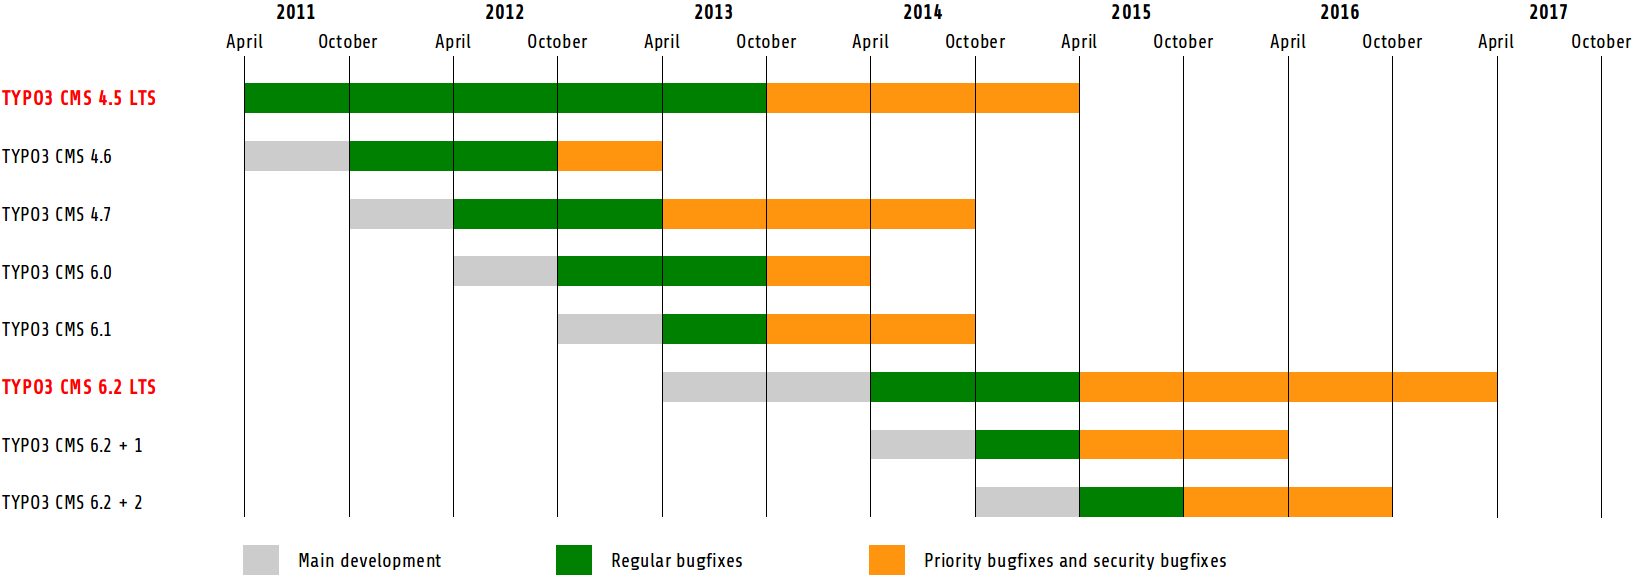
\includegraphics[width=0.90\linewidth]{Introduction/ReleaseAgenda.png}
	\end{figure}

\end{frame}

% ------------------------------------------------------------------------------
% LTXE-SLIDE-START
% LTXE-SLIDE-UID:		2bc48c66-067ca2a1-6d43b6d4-fe590a3e
% LTXE-SLIDE-ORIGIN:	855168a2-d07a3cc8-65f8f9bd-827ef9e9 English
% LTXE-SLIDE-TITLE:		TYPO3 CMS Roadmap
% ------------------------------------------------------------------------------
% https://typo3.org/typo3-cms/roadmap/

\begin{frame}[fragile]
	\frametitle{Introduzione}
	\framesubtitle{TYPO3 CMS Roadmap}

	Date di rilascio stimate e loro obiettivo principale:

	\begin{itemize}
		\item v7.0 \textrightarrow\tabto{1.3cm}02/Dec/2014\tabto{3.4cm}Revisione Backend Vol 1

		\item
			\begingroup
				\color{typo3orange}
					v7.1 \textrightarrow\tabto{1.3cm}24/Feb/2015\tabto{3.4cm}Pulizia core \& ottimizzazioni
			\endgroup

		\item v7.2 \textrightarrow\tabto{1.3cm}10/Mar/2015\tabto{3.4cm}Frontend
		\item v7.3 \textrightarrow\tabto{1.3cm}21/Apr/2015\tabto{3.4cm}Ecosistema Composer
		\item v7.4 \textrightarrow\tabto{1.3cm}09/Jun/2015\tabto{3.4cm}Revisione Backend Vol 2
		\item v7.5 \textrightarrow\tabto{1.3cm}28/Jul/2015\tabto{3.4cm}\textit{(da determinare...)}
		\item v7.6 \textrightarrow\tabto{1.3cm}13/Oct/2015\tabto{3.4cm}pre-LTS inferno
		\item v7.7 \textrightarrow\tabto{1.3cm}xx/xxx/2015\tabto{3.4cm}\textbf{TYPO3 CMS 7 LTS} (Long Term Release)
	\end{itemize}

	\smaller
		\url{https://typo3.org/typo3-cms/roadmap/}\newline
		\url{http://typo3.org/news/article/embrace-and-innovate-typo3-cms-7/}
	\normalsize

\end{frame}

% ------------------------------------------------------------------------------
% LTXE-SLIDE-START
% LTXE-SLIDE-UID:		3f43a11e-6ac44066-09edef27-24e867ec
% LTXE-SLIDE-ORIGIN:	0a54fbe0-06a2837d-605a5eed-6aa40506 English
% LTXE-SLIDE-TITLE:		Installation
% LTXE-SLIDE-REFERENCE:	https://forge.typo3.org/issues/62578
% ------------------------------------------------------------------------------

\begin{frame}[fragile]
	\frametitle{Introduzione}
	\framesubtitle{Installazione}

	\begin{itemize}
		\item Procedura ufficiale di installazione su Linux/Mac OS X\newline
			(DocumentRoot ad esempio \texttt{/var/www/site/htdocs}):
		\begin{lstlisting}
			$ cd /var/www/site
			$ wget --content-disposition get.typo3.org/7.1
			$ tar xzf typo3_src-7.1.0.tar.gz
			$ cd htdocs
			$ ln -s ../typo3_src-7.1.0 typo3_src
			$ ln -s typo3_src/index.php
			$ ln -s typo3_src/typo3
			$ touch FIRST_INSTALL
		\end{lstlisting}

		\item Link simbolici in Microsoft Windows:

			\begin{itemize}
				\item Use \texttt{junction} in Windows XP/2000
				\item Use \texttt{mlink} in Windows Vista and Windows 7
			\end{itemize}

	\end{itemize}
\end{frame}

% ------------------------------------------------------------------------------
% LTXE-SLIDE-START
% LTXE-SLIDE-UID:		45e1eb28-b0669fff-6c66805e-6e06b8cb
% LTXE-SLIDE-ORIGIN:	914dda49-a07eaf35-b9d24c58-6890a673 English
% LTXE-SLIDE-TITLE:		Upgrade to TYPO3 CMS 7
% LTXE-SLIDE-REFERENCE:	https://forge.typo3.org/issues/62578
% ------------------------------------------------------------------------------

\begin{frame}[fragile]
	\frametitle{Introduzione}
	\framesubtitle{Aggiornamento a TYPO3 CMS 7.x}

	\begin{itemize}
		\item Aggiornamenti possibili solo da TYPO3 CMS 6.2 LTS
		\item TYPO3 CMS < 6.2 deve essere prima aggiornato a TYPO3 CMS 6.2 LTS
	\end{itemize}

	\begin{itemize}

		\item Istruzioni per l'aggiornamento:\newline
			\smaller\url{http://wiki.typo3.org/Upgrade#Upgrading_to_7.1}\normalsize
		\item Guida ufficiale TYPO3 "TYPO3 Installation and Upgrading":
			\smaller\url{http://docs.typo3.org/typo3cms/InstallationGuide}\normalsize
		\item Approcio generale:
			\begin{itemize}
				\item Verifica i requisiti minimi di sistema \small(PHP, MySQL, etc.)
				\item Verifica \textbf{deprecation\_*.log} nella vecchia istanza TYPO3
				\item Aggiorna tutte le estensioni all'ultima versione
				\item Imposta il nuovo sorgente ed esegui Install Tool \textrightarrow Upgrade Wizard
				\item Verifica modulo startup per gli utente di backend (opzionale)
			\end{itemize}
	\end{itemize}

\end{frame}

% ------------------------------------------------------------------------------
